\chapter{The Conical Shape as the 3D Envelope of the Spiral}\label{sec:kegel}

\begin{figure}[t]
  \centering
  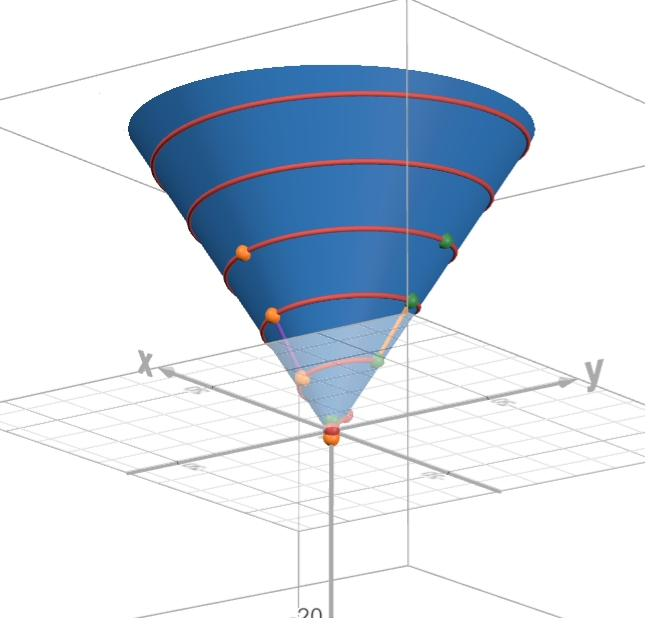
\includegraphics[width=0.72\textwidth]{bilder/Helix_3d}
  \caption{The conical helix: The red spiral curve winds upward along the blue
    cone surface $z = -\tfrac{3}{4} + \tfrac{\pi}{2}\,r$. The
    orange points mark the integer values $k(n)$ at
    $n \equiv 1 \pmod{6}$, the green points the values at
    $n \equiv 5 \pmod{6}$. The apex of the cone is located at
    $P_0 = (0,\,0,\,-\tfrac{3}{4})$; the
    light triangle in the foreground shows the radial cross-section and illustrates
    the constant slope $\Delta z / \Delta r = \pi/2$ of the generatrix.}
  \label{fig:kegelhelix_main}
\end{figure}

\section{From the 2D Model to the Conical Shape}

The spiral investigated previously possesses a pronounced arithmetic structure:
The points $P_n$ lie on radii whose distances are determined by the quadratic sequence
\[
k(n) = \frac{2n^2 + 3n + 1}{6}.
\]
Of particular importance are the values
\[
n \equiv 1,5 \pmod{6},
\]
for which the mean values $k(n)$ are integers. These two classes form an
alternating ray system that repeats every six steps.

The observation that these rays exhibit a regular structure in the plane
naturally leads to the question of whether there exists a three-dimensional shape
that geometrically consolidates this structure. The answer is a cone: It forms
an envelope in which the alternating rays appear as lines on the lateral surface
and the spiral itself can be interpreted as a space curve on this surface.

\section{3D Shape as a Right Circular Cone}

The three-dimensional structure arises from a geometrically unique
process. The starting point is the two-dimensional term curve
\[
r = r(p), \qquad \varphi = \varphi(p),
\]
whose trajectory we cut along the vertical axis. If this
curve segment is erected perpendicular to the plane and subsequently
wound spirally about the $z$-axis along its length, a
three-dimensional surface emerges whose generatrix is a straight line -- a
\emph{right circular cone}.

This can be justified as follows:

\begin{itemize}
  \item The radial increments of the sequence are constant:
  \[
  \Delta r = \frac{12}{\pi}.
  \]
  A surface on which equal radial increments lie along a fixed direction
  is necessarily a conical surface.

  \item The sequence possesses a periodic structure with
  \[
  \Delta n = 6.
  \]
  This periodicity is translated into a constant slope along the
  height during the winding process.

  \item Winding a planar curve with constant radial increment produces
  a surface whose generatrix is a straight line. This is precisely the defining
  property of a cone.
\end{itemize}

Hence the three-dimensional shape is a direct geometric consequence of winding the 2D curve. The spiral that arises on this surface is therefore a \emph{conical helix}, and the cone
itself is the natural envelope of the original two-dimensional structure.

\section{Radial Structure and Period-6 Periodicity}

Between two rays of the same class (i.e., two values $n$ with
$n \equiv 1 \pmod{6}$ or two values with $n \equiv 5 \pmod{6}$) there always lies
\[
\Delta n = 6.
\]

The corresponding radial spacing of the spiral is
\[
\Delta r = \frac{12}{\pi}.
\]

These two values form the foundation of the cone geometry: They determine the
slope of the cone and hence its opening angle.

\section{Derivation of the Cone Slope}

We consider the cross-section of the cone with a plane through the axis of rotation.
This produces a right triangle with
\[
\text{horizontal leg: } \Delta r = \frac{12}{\pi}, \qquad
\text{vertical leg: } \Delta z = 6.
\]

The slope of the cone follows from the ratio
\[
\frac{\Delta z}{\Delta r}
= \frac{6}{12/\pi}
= \frac{\pi}{2}.
\]

Thus the generatrix of the cone in the $(r,z)$-cross-section has the equation
\[
z = \frac{\pi}{2}\,r + b.
\]

\section{The Vertex of the Quadratic Sequence as the Cone Apex}

The constant $b$ follows directly from the structure of the quadratic sequence.
The vertex of the parabola
\[
k(n) = \frac{2n^2 + 3n + 1}{6}
\]
lies at
\[
n_0 = -\frac{3}{4}.
\]

This value marks the natural origin of the construction: It is the
point of minimal slope of the sequence and hence the geometric starting point of the
conical projection.

We identify
\[
z_0 = n_0 = -\frac{3}{4}, \qquad r_0 = 0.
\]

The point $(0,-\tfrac{3}{4})$ must therefore lie on the cone. Substitution into the
cone equation yields
\[
-\frac{3}{4} = \frac{\pi}{2}\cdot 0 + b,
\]
hence
\[
b = -\frac{3}{4}.
\]

This gives the definitive cone equation:
\[
\boxed{
z = -\frac{3}{4} + \frac{\pi}{2}\,r
}
\]

\section{Cone Surface and Generatrix}

The cone surface is the set of all points $(r,\varphi,z)$ satisfying the linear
relation between radius and height:
\[
z(r) = -\frac{3}{4} + \frac{\pi}{2}\,r.
\]

Each straight line on the surface corresponds to a fixed angular direction $\varphi$.
The alternating rays of the sequence lie exactly on such generatrices.
Their period-6 periodicity is encoded by the constant slope of the cone.

\section{Verification: The Conical Helix Lies Entirely on the Cone Surface}

\begin{theorem}[The Helix Lies on the Cone]
\label{satz:helixaufkegel}
The conical helix defined in Chapter~\ref{sec:helix},
\[
\gamma(\theta)
= \Bigl(\tfrac{6}{\pi^2}\theta\cos\theta,\;
        \tfrac{6}{\pi^2}\theta\sin\theta,\;
        -\tfrac{3}{4}+\tfrac{3}{\pi}\theta\Bigr),
\]
lies entirely on the cone surface
$z = -\tfrac{3}{4} + \tfrac{\pi}{2}\,r$ for all $\theta \geq 0$.
\end{theorem}

\begin{proof}
We must show that the $z$-coordinate of the helix equals
$-\tfrac{3}{4} + \tfrac{\pi}{2}\,r(\theta)$. We have:
\[
  r(\theta) = \frac{6}{\pi^2}\,\theta,
\]
hence
\[
  -\frac{3}{4} + \frac{\pi}{2}\,r(\theta)
  = -\frac{3}{4} + \frac{\pi}{2}\cdot\frac{6}{\pi^2}\,\theta
  = -\frac{3}{4} + \frac{3}{\pi}\,\theta
  = z(\theta). \qedhere
\]
\end{proof}

\begin{remark}
The identity $\frac{\pi}{2}\cdot\frac{6}{\pi^2} = \frac{3}{\pi}$ is the
algebraic core of the entire 3D model: The cone slope $\frac{\pi}{2}$
and the spiral parameter $a = \frac{6}{\pi^2}$ are precisely matched
so that the height function $z = \frac{3}{\pi}\theta$ emerges.
This relation follows from the choice $\Delta z = 6$ and
$\Delta r = \frac{12}{\pi}$, since
\[
  \frac{\Delta z}{\Delta r} = \frac{6}{12/\pi} = \frac{\pi}{2}
  \qquad\text{and}\qquad
  \frac{\pi}{2}\cdot a = \frac{\pi}{2}\cdot\frac{6}{\pi^2} = \frac{3}{\pi}.
\]
In Chapter~\ref{sec:visualisierung}, this cone conformity is verified purely
algebraically via the universal quantity $Q(k) = \sqrt{48k+1}$
(Theorem~\ref{satz:kegel}).
\end{remark}
